\documentclass[11pt]{article}

% Impostazioni del documento
\usepackage[a4paper,top=2cm,bottom=2cm,left=1cm,right=1cm,marginparwidth=2.5cm]{geometry}
\usepackage{parskip} % Spazio tra i paragrafi
\usepackage{setspace} % Interlinea
\onehalfspacing% Interlinea 1.5

% Impostazioni del font
\usepackage{mathptmx} % Times New Roman
\usepackage[T1]{fontenc}

% Altri
\usepackage{multicol}
\usepackage{graphicx}
\usepackage{enumitem}
\usepackage{hyperref}
\hypersetup{
    colorlinks=true,    % Rendi i link colorati
    linkcolor=blue,     % Colore dei link interni (es. sezioni)
    citecolor=blue,     % Colore delle citazioni bibliografiche
    urlcolor=blue       % Colore degli URL
}

\usepackage[style=numeric, backend=biber]{biblatex}

\usepackage{listings}
\usepackage{graphicx}
\usepackage{xcolor}

\lstset{
  language=C++,
  backgroundcolor=\color{black!5}, % imposta il colore di sfondo
  basicstyle=\footnotesize, % imposta la dimensione del carattere di base
  breaklines=true, % consente la rottura automatica delle righe
  keywordstyle=\color{blue}, % imposta il colore delle parole chiave
  commentstyle=\color{green}, % imposta il colore dei commenti
  stringstyle=\color{red}, % imposta il colore delle stringhe
  numbers=left, % mostra i numeri di riga a sinistra
}


\addbibresource{Bib.bib} % Specifica il tuo file .bib

\begin{document}

\begin{titlepage}
    \centering
    
\includegraphics[width=0.5\textwidth]{aau.png}
    \vfill
    \begin{center}
        {\LARGE C++ for High-Performance Computing \par}
        \vspace{0.5cm}
        {\large Alessandro Castelli [12246581] \par}
        \vspace{0.5cm}
        {\large \today \par}
    \end{center}
    \vfill
\end{titlepage}

\begin{multicols*}{2}[\columnsep=1cm]
    
    \section{Introduzione}
    In questo elaborato, saranno analizzati e discussi tre articoli che trattano dell'utilizzo del linguaggio di programmazione \texttt{C++} nel contesto del calcolo ad alte prestazioni.
    I tre articoli esaminano il tema da prospettive diverse. Gli articoli selezionati sono i seguenti:
    \begin{enumerate}
        \item \textit{C++ Reflection for High Performance Problem Solving Environments}~\cite{Article1}, reperibile al seguente link: \href{https://citeseerx.ist.psu.edu/document?repid=rep1&type=pdf&doi=2058bb40e6b80504ba1084452fd9c126cd19f891}{https://citeseerx.ist.psu.edu}
        \item \textit{How Templates Enable High-Performance Scientific Computing in C++}~\cite{Article2}, reperibile al seguente link: \href{https://ieeexplore.ieee.org/abstract/document/774843?casa_token=YqZfo7t12KoAAAAA:aUt-msPVNEAtzfVwO4h_-R_r7IPTFs7vHYHbAtsOdDE83PlNvB8gkNl5maWpHYBU5QkS3cUp0R8}{https://ieeexplore.ieee.org}
        \item \textit{Conduit: A C++ Library for Best-Effort High Performance Computing}~\cite{Article3}, reperibile al seguente link: \href{https://dl.acm.org/doi/abs/10.1145/3449726.3463205}{https://dl.acm.org}
    \end{enumerate}
    
    Ciascuno di questi documenti si occupa di affrontare problemi in ambienti ad alte prestazioni. In particolare, il primo articolo presenta un sistema di riflessione per il linguaggio C++, il quale consente la manipolazione dinamica di oggetti e funzioni del programma durante l'esecuzione. Il secondo articolo tratta dell'utilizzo del linguaggio C++ nello sviluppo di codice scientifico flessibile e ad alte prestazioni, sfruttando le potenti funzionalità dei template. Il terzo articolo introduce \texttt{Conduit}, una libreria C++ che fornisce un'interfaccia per implementare software che fa uso di comunicazione inter-thread e inter-processo a "miglior sforzo". Il concetto di "miglior sforzo" è una strategia che riduce la sincronizzazione e i requisiti di affidabilità dell'hardware, accettando il non determinismo in cambio di efficienza.
    Nel seguito del documento, verranno esposti gli argomenti trattati nei singoli articoli insieme alle relative metodologie, risultati e considerazioni critiche sulle implementazioni proposte.

    \section{C++ Reflection for High Performance Problem Solving Environments}
    L'articolo discute l'importanza degli Ambienti di Risoluzione dei Problemi (PSE), sistemi informatici che forniscono le risorse necessarie per risolvere specifiche classi di problemi. Tali PSE dovrebbero includere metodi avanzati di soluzione, selezione automatica o semi-automatica dei metodi, e la capacità di incorporare nuovi approcci.
    Nel calcolo scientifico, i PSE devono affrontare compiti intensivi in termini di CPU, spesso sviluppati come componenti in linguaggi ad alte prestazioni. L'articolo sostiene che i PSE dovrebbero consentire il dinamico accoppiamento di compiti, con un'interfaccia utente grafica o uno scripting ambiente. Tuttavia, la mancanza di riflessione nei moderni linguaggi HPC porta gli sviluppatori di PSE a dipendere da linguaggi come Java, causando inconvenienti.
    L'articolo propone l'implementazione di funzionalità (di una libreria) di riflessione non invasiva e conformi agli standard in C++, dimostrando che questo può essere fatto in modo efficiente. Confronta il sovraccarico della riflessione con altri metodi e suggerisce che la sua implementazione è l'unico modo per incorporare funzionalità di riflessione in C++ in modo conforme agli standard e non invasivo.
    L'articolo discute i due tipi di riflessione a livello di codice: in fase di compilazione e in fase di esecuzione. La riflessione in fase di compilazione consente l'accesso alle informazioni sul tipo durante la compilazione, facilitando la programmazione generica, mentre la riflessione in fase di esecuzione offre la capacità di accedere dinamicamente alle informazioni sul tipo durante l'esecuzione del programma.
    Mentre linguaggi come Java, C\# e Python supportano la riflessione come parte delle loro specifiche standard, C++ fornisce solo funzionalità limitate tramite le informazioni sul tipo in fase di esecuzione (RTTI). Visual C++ ha estensioni per la riflessione, ma con limitata portabilità. Per l'elaborazione ad alte prestazioni, Java e C\# sono limitati, mentre Fortran domina, ma C++ è preferito per il middleware.
    La riflessione in fase di esecuzione richiede la generazione separata di metadati come codice C++ effettivo, poiché i compilatori C++ non generano automaticamente i metadati richiesti. L'articolo propone che C++ dovrebbe supportare la riflessione in modo standard e non intrusivo, e mostra come questo può essere fatto in modo efficiente.
    
    \paragraph{Esempio preso dal documento:}
    Considera il seguente blocco di codice:
    \begin{lstlisting}
        classType = ClassType::getClass("Service1");
        obj = classType.createInstance();
        obj.invoke("method1");
    \end{lstlisting}

    L'uso della riflessione consente di incorporare dinamicamente moduli esistenti in un'applicazione in modo dinamico e flessibile. Ad esempio, considerando una funzione come \texttt{init\_lib()}, di solito richiederebbe la scrittura di codice specifico, ma con la riflessione, è possibile specificare il nome della funzione in un file di configurazione, consentendo la chiamata dinamica senza la necessità di scrivere nuovo codice o ricompilare. Questo approccio si estende anche ad altre funzioni del modulo, consentendo un incollaggio automatico tra moduli mediante l'uso di un'ontologia o una descrizione semantica. La riflessione diventa così uno strumento potente per lo sviluppo di codice riutilizzabile, semplificando il processo di integrazione di moduli esistenti in un'applicazione più ampia. Rendendo "Service1" e "method1" parametri configurabili, questo codice potrebbe essere utilizzato per invocare qualsiasi metodo.
    I maggiori vantaggi in questo sarebbero quindi:
    \begin{itemize}
        \item \textbf{Configurabilità dinamica:} Utilizzando la riflessione, è possibile specificare dinamicamente quali classi e metodi devono essere utilizzati senza dover modificare il codice sorgente. Ad esempio, nel blocco di codice fornito, il nome della classe ("Service1") e il nome del metodo ("method1") possono essere specificati in un file di configurazione anziché nel codice.
        \item \textbf{Integrazione di moduli esterni:} La riflessione semplifica l'integrazione di moduli esterni o librerie in un'applicazione senza la necessità di adattare il codice sorgente esistente. Ciò rende più facile aggiungere, rimuovere o sostituire funzionalità senza dover ricompilare l'applicazione principale.
        \item \textbf{Riusabilità del codice:} La riflessione può favorire la scrittura di codice più generico e riusabile. Nel caso di funzioni come "init\_lib()", la capacità di chiamare dinamicamente funzioni in base al loro nome semplifica l'utilizzo di moduli senza dover scrivere codice specifico per ciascuna funzione.
        \item \textbf{Facilità nell'aggiornamento e manutenzione:} Se si utilizza la riflessione per gestire dinamicamente le funzionalità dell'applicazione, può diventare più semplice aggiornare o modificare parti dell'applicazione senza impattare altre parti del codice.
    \end{itemize}
    \paragraph{Riflessione: Idee su come può essere applicata}
    Il documento da alcune idee su come applicare la riflessione utilizzando diverse tecniche, di seguito troverai diversi contesti e casi d'uso in cui la riflessione viene implementata o sfruttata per ottenere determinati vantaggi o funzionalità.
    \begin{itemize}
    \item {Serializzazione:}
    Il processo di serializzazione, che consiste nel convertire lo stato di un oggetto in una sequenza di byte e successivamente deserializzarlo, è un metodo comune per la comunicazione tra applicazioni poco accoppiate. 
    Nel contesto di un PSE, questa sequenza di byte può essere impiegata per trasferire dati dall'output di un'attività all'input di un'altra. 
    Utilizzando la riflessione, il mittente può serializzare dinamicamente lo stato di un oggetto e inviarlo al ricevente, il quale può creare gli oggetti dinamicamente basandosi sulle loro descrizioni e popolarli con le informazioni sullo stato corrispondente. 
    \item {Interfaccia a un Ambiente di Scripting:}
    Nel contesto della riflessione e dell'interfaccia a un ambiente di scripting, l'obiettivo è consentire agli utenti di uno scripting language, come Python, di utilizzare funzionalità implementate in linguaggi ad alte prestazioni come C, C++ o Fortran senza la necessità di riscrivere completamente il codice in uno scripting language.
    Le librerie ad alte prestazioni, scritte in linguaggi come C, C++ o Fortran, sono spesso utilizzate per compiti computazionali intensivi o per ottimizzare le prestazioni. Tuttavia, l'accesso diretto a queste librerie da parte di utenti che preferiscono linguaggi di scripting come Python potrebbe essere complesso a causa delle differenze nella gestione della memoria, nella sintassi e nella struttura dei linguaggi.
    La riflessione viene utilizzata per creare un'interfaccia tra queste librerie e l'ambiente di scripting. Ciò significa che, anziché richiedere agli utenti di scripting di scrivere wrapper o bindings complessi per chiamare le funzioni di queste librerie, la riflessione viene impiegata per fornire un meccanismo più automatico e meno oneroso.    
    \item {Istanziamento di Oggetti:}
    La riflessione è impiegata per risolvere il problema dell'istanziamento polimorfico degli oggetti, offrendo un'alternativa alla necessità di avere un metodo di fabbrica specifico per ogni classe. Questo approccio rende il processo di istanziazione più flessibile e meno intrusivo.
    Nel contesto dell'istanziamento polimorfico, la pratica comune è utilizzare il "factory method pattern", che richiede che ogni classe candidata implementi un metodo dedicato per la creazione di un nuovo oggetto del tipo richiesto. Questa procedura può risultare onerosa e intrusiva, specialmente quando si lavora con nuove classi o con classi già esistenti che devono essere adattate.
    Con l'impiego della riflessione, non sono richiesti i vincoli del "factory method pattern". Invece, è possibile istanziare gli oggetti dinamicamente, senza la necessità di implementare metodi di fabbrica specifici.
    \end{itemize}
    \paragraph{Obiettivi della Libreria di Riflessione in C++}

    \begin{enumerate}
        \item \textbf{Accesso a Runtime ai Membri:} Fornire la possibilità di accedere a runtime alle funzioni membro e ai membri di dati di una classe, consentendo l'invocazione di funzioni membro e la lettura/scrittura di membri di dati.
    
        \item \textbf{Completezza:} La libreria dovrebbe offrire informazioni complete sulle classi e i loro membri, consentendo un accesso dettagliato.
    
        \item \textbf{Conformità agli Standard:} Essere conforme allo standard ISO C++, garantendo la portabilità della libreria senza dipendere da caratteristiche non standard.
    
        \item \textbf{Efficienza:} Ridurre al minimo l'overhead dell'accesso alle classi e ai loro membri attraverso la riflessione. L'utilizzo di modelli C++ per registrare la maggior parte dei metadati a compile time contribuisce a garantire un codice risultante efficiente.
    
        \item \textbf{Non Intrusività:} Implementare la riflessione senza richiedere modifiche al codice esistente. Evitare l'aggiunta di annotazioni speciali alle classi esistenti per garantire una facile integrazione con il codice preesistente e ridurre il rischio di errori nelle sezioni di meta-informazioni.
    \end{enumerate}

    \subsection{Implementazione della libreria di riflessione in C++}
    La libreria è strutturata con un nucleo di classi di base e un insieme di classi generate per gestire le informazioni specifiche del tipo. Queste classi di metadati specifici del tipo vengono create mediante l'analisi delle classi di destinazione fornite dall'utente e la successiva elaborazione degli alberi sintattici. Questo approccio ci consente di memorizzare e presentare in modo efficiente le informazioni di riflessione senza essere invasivi e garantendo la conformità agli standard del linguaggio C++.
    \subparagraph*{Metaclasses}
    \texttt{ClassType} è la metaclasse utilizzata per rappresentare classi definite dall'utente. 
    Queste classi derivano da una classe più generica chiamata \texttt{Type} (Guarda figura \ref*{fig:ClassType}).
    
    \texttt{ClassType}, insieme alle sue classi di supporto, fornisce le seguenti caratteristiche:
        \begin{itemize}
            \item Nome e tipo
            \item Lista di membri dati e funzioni membro
            \item Interfaccia di istanziazione
            \item Informazioni sull'ereditarietà
        \end{itemize}
    Dopo aver creato un'istanza di \texttt{ClassType}, l'oggetto di destinazione effettivo può essere creato.
    Gli altri tipi derivati, \texttt{FundamentalType}, \texttt{ArrayType} e \texttt{PointerType}, come suggeriscono i loro nomi, sono utilizzati per rappresentare tipi primitivi (ad esempio, integer, double), array e puntatori.

    \paragraph{Member Classes}
    Ci sono due tipi di classi membro, ovvero membri dati e funzioni membro. Queste encapsulano i membri di una classe e forniscono mezzi per accedervi in modo indiretto, dato il loro nome a tempo di esecuzione. Invece di mantenere l'offset al membro encapsulato, ogni classe membro mantiene un puntatore al suo rispettivo membro dati o funzione membro. Ciò assicura che questa libreria sia completamente conforme allo standard C++.
    \subparagraph*{Data Members}
    Ogni membro dati in una classe è rappresentato da un oggetto DataMember. Questo oggetto contiene informazioni come nome e tipo.
    Il metodo ref() restituisce un riferimento all'oggetto rappresentato, consentendo al programma di manipolarlo come se avesse accesso diretto al membro dati.
    BoundDataMember è consapevole dell'oggetto associato, eliminando la necessità di passare un riferimento a classAObj. I membri dati vincolati sono ora completamente indipendenti dal tipo sottostante, rendendoli adatti a codice completamente generico.

    \subparagraph*{Member Functions}
    Le funzioni membro sono rappresentate dalle classi \texttt{MemberFunction}, che forniscono informazioni come nome, tipo di ritorno e interfacce aggiuntive.
    Gli argomenti delle funzioni membro sono gestiti come un vettore di oggetti generici di tipo (Type), consentendo la rappresentazione di tipi fondamentali, puntatori, array e classi definite dall'utente.
    L'invocazione di funzioni membro può avvenire in due modi: uno richiede l'invio degli argomenti singolarmente con un puntatore all'istanza corrispondente, l'altro accetta un vettore di argomenti.

    \paragraph{Performance}
    Dopo l'implementazione della libreria, sono stati condotti test al fine di valutare le prestazioni. Era atteso un calo di prestazioni, e l'obiettivo consisteva nel misurare l'incremento di tempo rispetto alle chiamate dirette. Ogni test coinvolgeva l'istanziazione dinamica di un oggetto e l'invocazione di un metodo su di esso, con cinque metodi che variavano nel numero di argomenti (da 1 a 5). I metodi sono stati invocati come chiamate dirette e virtuali, oltre che utilizzando la riflessione. Nel caso dell'uso della riflessione, l'istanza dell'oggetto è stata effettuata mediante metodi riflessivi. L'attenzione principale era focalizzata sul rilevamento del sovraccarico nell'uso della riflessione in confronto alle chiamate dirette, calcolando questo sovraccarico come il tempo aggiuntivo in percentuale rispetto alle chiamate dirette.
    Quello che è possibile osservare dai test è che il sovraccarico per la riflessione in C++ aumenta con il numero di argomenti. Questo è principalmente dovuto alla costruzione dinamica della lista degli argomenti, che comporta poche piccole allocazioni di memoria. 
    \subsection{My vision}
    Lo sviluppo di questa libreria ha secondo me molti spunti interessanti. Di seguito elencherò alcuni punti che riassumono le mia vissione con dei possibili miglioramenti.
    \begin{itemize}
        \item \textbf{Arricchimento delle Funzionalità:} L'obiettivo primario è di arricchire la libreria di riflessione introducendo nuove funzionalità che ne amplifichino la potenza e l'estensibilità. In questo contesto, valutiamo attentamente l'inclusione di supporto per la gestione di attributi personalizzati, l'implementazione di una navigazione avanzata della gerarchia delle classi e lo sviluppo di strumenti per la manipolazione avanzata dei tipi.
        \item \textbf{Ottimizzazione delle Performance:} Dedichiamo particolare attenzione all'ottimizzazione delle prestazioni con l'obiettivo di ridurre ulteriormente l'overhead introdotto durante l'invocazione di funzioni membro e l'accesso ai membri dati. Mantenendo un focus costante sull'efficienza, ci proponiamo di garantire che la libreria possa essere utilizzata in contesti ad alte prestazioni senza compromettere la sua efficienza.
        \item \textbf{Integrazione con Tecnologie Esterne:} Esploriamo attivamente opportunità di integrazione con tecnologie e framework ampiamente adottati. La libreria potrebbe trarre beneficio da una maggiore compatibilità con sistemi di serializzazione/deserializzazione diffusi o ambienti di scripting, aprendo nuove possibilità di utilizzo in scenari complessi e eterogenei.
        \item \textbf{Ampio Supporto per Compilatori:} Ci impegniamo a garantire che la libreria sia compatibile con una vasta gamma di compilatori C++. L'obiettivo è estendere il supporto oltre ai compilatori attualmente considerati, assicurando che la libreria sia accessibile a un pubblico più ampio di sviluppatori che utilizzano una varietà di ambienti di sviluppo.
        \item \textbf{Documentazione Approfondita e Accessibile:} Investiamo nella creazione di una documentazione completa, chiara e accessibile. La documentazione sarà arricchita da esempi pratici, scenari d'uso dettagliati e spiegazioni tecniche. Questo sforzo mira a guidare gli sviluppatori, sia principianti che esperti, nell'uso efficace della libreria, contribuendo così alla sua adozione e successo nella community.
        \item \textbf{Rigore nei Test e nella Validazione:} Implementiamo un sistema completo di test e validazione per garantire che la libreria funzioni correttamente in varie situazioni e configurazioni. Attraverso questo approccio rigoroso, miriamo a mantenere la stabilità e l'affidabilità della libreria nel tempo, fornendo agli sviluppatori la fiducia necessaria nell'integrazione e nell'uso della libreria.
    \end{itemize}

\section{How templates enable high-performance scientific computing in C++}
    Il linguaggio di programmazione C++ offre una potente struttura di templates, consentendo lo sviluppo di software flessibile senza sacrificare prestazioni. I templates permettono di definire classi e funzioni parametrizzate in termini di altri tipi e costanti. Questa caratteristica è fondamentale per la costruzione di codici scientifici astratti e ad alte prestazioni in C++. Il framework Pooma è citato come esempio, supportando il calcolo scientifico ad alte prestazioni e fornendo astrazioni matematiche e fisiche avanzate. 
    Pooma permette una transizione agevole tra esecuzione seriale e parallela su diverse piattaforme, inclusa la supercomputing.
    \paragraph{Come funzionano i template in C++}
    Di seguito troverai un esempio banale di come possono essere utili i templates.
    \begin{lstlisting}[language=C++, label=code1, caption={Max function without template}]
    {
    if (a > b) return a;
    else return b;
    }
    \end{lstlisting}
    Se avessimo bisogno di scrivere una versione per float, double o qualsiasi altro tipo aritmetico, il codice sarebbe esattamente lo stesso. Invece di riprodurre questo codice per ogni tipo, possiamo scrivere una funzione template (Listing \ref{code2}) per generare una funzione più generale.
    
    \begin{lstlisting}[language=C++, label=code2, caption={Max function with template}]
    template <class T>
    T max(T a, T b)
    {
    if (a > b) return a;
    else return b;
    }
    \end{lstlisting}
    
    Il simbolo T è un parametro del template in C++, e la sintassi "class T" può essere fuorviante perché T non deve necessariamente rappresentare una classe C++. Gli argomenti del template possono essere specificati in modo esplicito, ad esempio con `max<int>(3, 2)`, dove il compilatore crea una versione concreta di max sostituendo int a T. Tuttavia, è più comune consentire al compilatore di dedurre il tipo osservando gli argomenti, come nel caso di `max(3.0, 2.0)`, dove il compilatore genererà una versione di max con double sostituito a T.
    Questa deduzione del tipo non è una semplice sostituzione testuale come avverrebbe con un preprocessore di macro. T è atteso abbia la semantica di un tipo, permettendo la dichiarazione di oggetti di quel tipo, come evidenziato negli argomenti e nel valore di ritorno della funzione max. In sintesi, l'utilizzo di template in C++ consente una flessibilità notevole nella creazione di funzioni e classi generiche, con la deduzione del tipo da parte del compilatore che contribuisce alla semplicità e alla chiarezza del codice.

    \subsection{Pooma}
    \paragraph{Array Concept}
    Quando utilizzato da solo, un array si riferisce a tutti i alori del suo dominio e a cui possono venire applicate operazioni matematica o funzioni elementari.
    Un Array in Pooma può avere fino a sette dimensioni e possono fungere da contenitori per tipi arbitrari. 
    Il concetto di Array di Pooma supporta domini più complessi ed inoltre, l'indicizzazione degli Array in Pooma è polimorfica; cioè, l'operazione di indicizzazione \texttt{X(i1, i2)} può eseguire la mappatura da dominio a intervallo in una varietà di modi, a seconda del tipo specifico dell'Array che viene indicizzato.
    Analizziamo il modello del concetto di Array in Pooma, il template di classe Array.
    Le tre richieste più importanti dal punto di vista del design generale sono:
    • dominio arbitrario,
    • intervallo arbitrario, e
    • indicizzazione polimorfica.
    Il template della classe Array in Pooma permette di creare diverse classi Array, ognuna con un diverso numero di dimensioni (Dim), tipo di elementi (T) e modalità di indicizzazione (EngineTag). Questa flessibilità consente di definire array con domini arbitrari, intervalli di output arbitrari e diversi modi di indicizzazione, contribuendo a un design generale versatile ed efficiente.
    
    \paragraph{Engine}
    Il concetto di "Engine" in Pooma è fondamentale per l'indicizzazione polimorfica nella gestione degli array multidimensionali. La classe "Array" delega la memorizzazione e la ricerca dei dati a un oggetto "Engine", il cui design è guidato da requisiti specifici per essere considerato un modello del concetto di Engine.

    La classe "Array" è parametrizzata da tre template: Dim (dimensione del dominio), T (tipo degli elementi dell'array) e EngineTag (modalità di indicizzazione). Questa parametrizzazione consente la creazione di diverse classi Array con caratteristiche specifiche, promuovendo un design flessibile e efficiente.

    Il concetto di Engine è definito dai requisiti imposti dalla classe Array al suo motore. In particolare, il motore deve essere una specializzazione di un template generale "Engine" con parametri identici a quelli della classe Array. Deve inoltre definire pubblicamente un tipo chiamato "Index\_t" e fornire una versione dell'operatore "()” che accetta indici di tipo "Index\_t".

    L'indirezione tra Array ed Engine consente a Pooma di supportare l'indicizzazione polimorfica. Ad esempio, se il motore lavora con un dominio discreto, definisce "Index\_t" come un tipo integrale; se lavora con un dominio continuo, definisce "Index\_t" come un tipo in virgola mobile.

    La classe "Array" utilizza l'operatore "()” per passare gli indici al suo oggetto "Engine". Questa separazione consente a Array di essere un modello fedele del concetto di Array, offrendo un'ampia varietà di costruttori, operatori sovraccaricati e supporto per espressioni. Al contrario, gli oggetti Engine sono interfaccia a basso livello per una sorgente dati utente-definita, con accesso diretto ai dati gestito da Array.

    L'approccio di Pooma, basato sulla separazione di interfaccia e implementazione, offre una maggiore complessità e ricchezza di funzionalità nella classe Array rispetto agli oggetti Engine, consentendo una facile estensione e personalizzazione da parte degli utenti.
    
    \subsection{Compile-time versus runtime polymorphism}
    Il confronto tra polimorfismo a tempo di compilazione e a tempo di esecuzione evidenzia le differenze cruciali in termini di flessibilità ed efficienza nell'implementazione del concetto di Engine in Pooma.
    L'articolo mette in evidenza il polimorfismo a tempo di compilazione, sottolineando che la conoscenza dei tipi durante la compilazione consente ottimizzazioni rilevanti. Viene confrontato con un'implementazione a tempo di esecuzione, evidenziando le limitazioni di flessibilità ed efficienza di quest'ultima.

    La conclusione sottolinea che l'approccio a tempo di compilazione, mediante classi template e motori, offre una soluzione più flessibile ed efficiente rispetto a un'implementazione a tempo di esecuzione basata su ereditarietà e funzioni virtuali. Questa analisi può essere utile per comprendere le scelte di progettazione nell'implementazione di array multidimensionali in contesti scientifici.
    \subsection{My Vision}
    Nella mia visione personale, l'utilizzo dei template in C++ per il calcolo scientifico rappresenta un passo significativo verso la creazione di codice più flessibile, efficiente e facilmente manutenibile. L'approccio di parametrizzazione dei tipi offerto dai template consente agli sviluppatori di scrivere codice generico che può essere applicato a una vasta gamma di tipi di dati, contribuendo così alla creazione di librerie e framework riutilizzabili.
    Il framework Pooma, come esemplificato nel paper, dimostra come l'uso intelligente dei template può fornire un'astrazione potente per il calcolo scientifico ad alte prestazioni. La possibilità di gestire la transizione tra esecuzione seriale e parallela su diverse piattaforme, inclusa la supercomputing, evidenzia l'adattabilità e la portabilità che i template possono offrire in contesti scientifici complessi.
    Inoltre, l'analisi del polimorfismo a tempo di compilazione rispetto a quello a tempo di esecuzione sottolinea l'importanza di considerazioni di prestazioni e flessibilità durante la progettazione di sistemi scientifici. La capacità di effettuare ottimizzazioni durante la compilazione, grazie alla conoscenza statica dei tipi, può portare a un codice più efficiente e adattabile alle esigenze specifiche delle applicazioni scientifiche.
    La mia visione sottolinea anche l'importanza di una comunità scientifica impegnata nel condividere best practices e esperienze nell'uso dei template. La collaborazione tra sviluppatori scientifici può contribuire alla creazione di linee guida e standard che facilitano l'adozione efficace dei template in vari contesti scientifici.

    In sintesi, la mia visione riflette l'entusiasmo per il potenziale dei template in C++ nel campo del calcolo scientifico e la convinzione che questa tecnologia possa continuare a guidare l'evoluzione di soluzioni software innovative e performanti.

\section{Conduit: A C++ Library for Best-effort High Performance Computing}
Il documento introduce le sfide nello sviluppo di software per sfruttare efficacemente la capacità crescente di elaborazione parallela e distribuita. 
Le tecniche tradizionali presuppongono la sincronizzazione tra esecuzione, comunicazione tra processi e gestione della memoria, ma ciò diventa costoso su larga scala. 
Viene proposta la strategia della \textbf{computazione best-effort}, che rilassa i requisiti di sincronizzazione e affidabilità hardware in cambio di efficienza.

La libreria \textbf{Conduit} in C++ si propone di fornire un'interfaccia preconfezionata per implementare software che utilizza la comunicazione best-effort tra thread e processi. 
Il documento copre motivazioni, obiettivi, design e implementazione della libreria. I benchmark su problemi di colorazione di grafi e simulazioni di evoluzione digitale dimostrano che il modello best-effort di Conduit può migliorare l'efficienza di scaling e la qualità delle soluzioni.
Viene introdotta l'idea di "computazione best-effort" dove si rilassano le dipendenze dati per ridurre la sincronizzazione, migliorando la scalabilità. Si menziona che gli algoritmi deterministici basati sulla sincronizzazione globale diventano costosi su sistemi di calcolo ad alte prestazioni. L'aspirazione alla scalabilità indefinita richiede operazioni asincrone, reti decentralizzate, componenti intercambiabili e degradazione graziosa in caso di guasti hardware.

\subsection{Conduit Library}
Conduit è una libreria C++ che mira ad integrarsi nei sistemi di programmazione parallela, fornendo un'interfaccia astratta di tipo best-effort agli sviluppatori.
La Figura \ref{fig:Conduit} fornisce una panoramica schematica di Conduit.
Quello che succede è che un Inlet e un Outlet possono scambiarsi messaggi tramite una procedura di comunicazione intra-thread, inter-thread o inter-processo, a seconda dello stato di runtime di un oggetto Duct sottostante e Conduit fornisce una libreria di implementazoine per fare ciò.

L'oggetto \textit{Inlet} fornisce due metodi principali: \texttt{TryPut()} e \texttt{Put()}. Il metodo \texttt{TryPut()} è non bloccante e cerca di mettere in coda un messaggio per il corrispondente \textit{Outlet}. In caso di sovraccarico, il messaggio può essere eliminato. D'altra parte, il metodo \texttt{Put()} si blocca in condizioni di sovraccarico, attendendo finché lo spazio nel buffer non è disponibile per accodare il messaggio.

Per quanto riguarda l'oggetto \textit{Outlet}, offre i metodi \texttt{TryStep()}, \texttt{Jump()} e \texttt{Step()}. I primi due metodi sono utilizzati per caricare il messaggio successivo o più recente, rispettivamente. Nel caso in cui non ci siano nuovi messaggi disponibili, verrà utilizzato l'ultimo messaggio ricevuto. Il metodo \texttt{Step()} si blocca fino a quando non viene ricevuto un nuovo messaggio.

A livello di runtime, gli oggetti \textit{Duct} possono essere creati o modificati per gestire la comunicazione intra-thread, inter-thread o inter-processo.

Oltre a questa interfaccia granulare a livello di connessione, Conduit fornisce un'interfaccia a livello di rete in cui l'utente definisce la propria computazione in termini di un grafo orientato.
Conduit non solo offre un'interfaccia granulare a livello di connessione, ma fornisce anche un'interfaccia a livello di rete in cui gli utenti definiscono la propria computazione utilizzando un grafo orientato. In questa topologia, i nodi rappresentano elementi di simulazione, mentre gli archi indicano canali di comunicazione.
La libreria assegna automaticamente nodi a thread disponibili su processi disponibili e istanzia i condotti corrispondenti. I singoli thread possono quindi elaborare liberamente gli aggiornamenti computazionali sui nodi loro assegnati, ricevendo contemporaneamente messaggi da nodi assegnati ad altri processi man mano che diventano disponibili. 
Definire la logica del programma in termini di elementi di simulazione atomici che comunicano offre notevoli vantaggi in termini di programmabilità. Questo approccio consente la scrittura del codice in termini di interazioni tra oggetti intuitivi specifici del dominio  con la gestione automatica della mappatura sulle risorse hardware da parte del framework sottostante.
Tuttavia, un'implementazione ingenua comporterebbe inefficienze significative, specialmente nella comunicazione inter-processo con un notevole overhead. 

\subsection{Metodologie usate per valutare le prestazioni}
Per verificare l'impatto sulle prestazioni dato dall'utilizzo della libreria Conduit sono stati fatti dei test che hanno seguito determinate metodologie.
Vengono eseguiti due benchmark per confrontare l'approccio best-effort di Conduit con un modello sincrono tradizionale. 
I benchmark vengono eseguiti sia in un contesto di memoria condivisa multithread che in un contesto distribuito multinode. 
In ciascun contesto hardware, le prestazioni vengono valutate su due contesti algoritmici: un problema di colorazione di grafi distribuiti intensivo in comunicazione e una simulazione di evoluzione digitale intensiva in calcolo.

Il benchmark relativo al problema di colorazione di grafi distribuiti è stato scelto per complementare il lavoro originale di sviluppo della libreria Conduit, al fine di supportare sistemi sperimentali su larga scala per lo studio dell'evoluzione aperta. Il benchmark relativo alla simulazione di evoluzione digitale è stato sviluppato per valutare le prestazioni della libreria in un contesto di calcolo intensivo.

\subsection{Performance}
Come già accennato, i benchmark sono stati eseguiti su due contesti algoritmici: un problema di colorazione di grafi distribuiti intensivo in comunicazione e una simulazione di evoluzione digitale intensiva in calcolo. I benchmark sono stati eseguiti sia in un contesto di memoria condivisa multithread che in un contesto distribuito multinode.

Nel contesto di memoria condivisa multithread, i risultati mostrano che le prestazioni della libreria Conduit diminuiscono con l'aumentare del numero di thread, ma che l'approccio best-effort di Conduit è comunque in grado di fornire prestazioni migliori rispetto al modello sincrono tradizionale. In particolare, il benchmark relativo al problema di colorazione di grafi distribuiti ha mostrato che l'approccio best-effort di Conduit ha permesso di ottenere una soluzione di qualità migliore rispetto al modello sincrono tradizionale, entro un determinato limite di tempo. Il benchmark relativo alla simulazione di evoluzione digitale ha mostrato che l'approccio best-effort di Conduit ha permesso di ottenere un aumento significativo delle prestazioni rispetto al modello sincrono tradizionale.

Nel contesto distribuito multinode, i risultati mostrano che l'approccio best-effort di Conduit è in grado di fornire prestazioni migliori rispetto al modello sincrono tradizionale, soprattutto in contesti di calcolo intensivo. In particolare, il benchmark relativo alla simulazione di evoluzione digitale ha mostrato che l'approccio best-effort di Conduit ha permesso di ottenere un aumento significativo delle prestazioni rispetto al modello sincrono tradizionale, con un speedup di circa 2,1x rispetto all'esecuzione completamente sincrona.

In generale, i risultati dei benchmark dimostrano che l'approccio best-effort di Conduit è in grado di fornire prestazioni migliori rispetto al modello sincrono tradizionale in contesti di calcolo ad alte prestazioni, soprattutto in contesti di calcolo intensivo. Gli autori del paper concludono che la libreria Conduit può essere utilizzata per ridurre le barriere di esperienza nel dominio e di programmabilità per sfruttare in modo efficiente la crescente potenza di calcolo parallelo e distribuito.

\subsection{My Vision}
Nel mio parere, l'articolo fornisce una visione interessante sull'implementazione di un'interfaccia best-effort per la comunicazione tra thread e processi in contesti di calcolo ad alte prestazioni. L'approccio best-effort presentato nella libreria Conduit sembra offrire vantaggi significativi in termini di prestazioni, soprattutto in contesti di calcolo intensivo e distribuito.
Tuttavia, ritengo che l'articolo potrebbe essere migliorato includendo una discussione più dettagliata sulle sfide e le limitazioni dell'approccio best-effort. Ad esempio, potrebbe essere utile esplorare in modo più approfondito i potenziali trade-off tra prestazioni e affidabilità nell'ambito dell'approccio best-effort, nonché le strategie per gestire eventuali perdite di dati o ritardi nella comunicazione.
Inoltre, sarebbe interessante vedere ulteriori esempi di casi d'uso pratici della libreria Conduit in contesti reali di calcolo ad alte prestazioni. Questi casi d'uso potrebbero aiutare a dimostrare l'efficacia e l'applicabilità dell'approccio best-effort in una varietà di scenari applicativi.
Infine, sarebbe utile includere una sezione dedicata alle future direzioni di ricerca e sviluppo per la libreria Conduit. Questa sezione potrebbe esplorare potenziali miglioramenti o estensioni della libreria, nonché possibili applicazioni in nuovi settori o domini di calcolo ad alte prestazioni.

In sintesi, l'articolo offre una visione promettente sull'implementazione di un'interfaccia best-effort per la comunicazione in contesti di calcolo ad alte prestazioni, ma potrebbe beneficiare di una maggiore approfondimento delle sfide e delle opportunità future.
\end{multicols*}

\begin{figure}
    \centering
    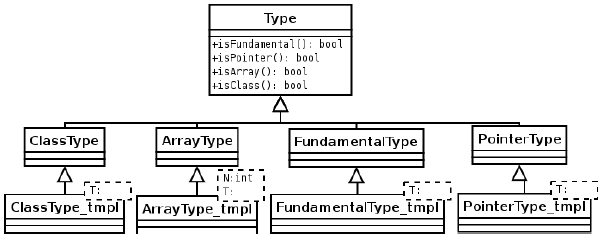
\includegraphics[width=0.5\linewidth]{ClassType.png}
    \caption{Metaclass hierarchy}
    \label{fig:ClassType}
\end{figure}

\begin{figure}
    \centering
    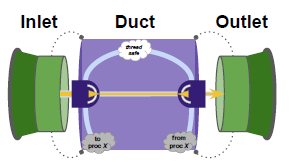
\includegraphics[width=0.5\linewidth]{Conduit.png}
    \caption{Conduit Scheme}
    \label{fig:Conduit}
\end{figure}

\printbibliography\end{document}
